\documentclass[iop,revtex4,natbib209]{emulateapj}

\usepackage[english]{babel}
\usepackage{natbib}
\usepackage{graphicx}
\usepackage[space]{grffile}
\usepackage{latexsym}
\usepackage{amsfonts,amsmath,amssymb}
\usepackage{url}
\usepackage[utf8]{inputenc}
\usepackage{fancyref}
\usepackage{hyperref}
\hypersetup{colorlinks=false,pdfborder={0 0 0},}
\usepackage{textcomp}
\usepackage{longtable}
\usepackage{multirow,booktabs}
\usepackage{pdflscape}
\usepackage{listings}
\usepackage{textcomp}
\usepackage[T1]{fontenc}
\usepackage[colorinlistoftodos,prependcaption,textsize=normal]{todonotes}

\newcommand{\vdag}{(v)^\dagger}

\newcommand{\truncateit}[1]{\truncate{0.8\textwidth}{#1}}
\newcommand{\scititle}[1]{\title[\truncateit{#1}]{#1}}

\usepackage{color}
 
\definecolor{codegreen}{rgb}{0,0.6,0}
\definecolor{codegray}{rgb}{0.5,0.5,0.5}
\definecolor{codepurple}{rgb}{0.58,0,0.82}
\definecolor{backcolour}{rgb}{0.95,0.95,0.92}
 
\lstdefinestyle{mystyle}{
    backgroundcolor=\color{white},   
    commentstyle=\color{codegreen},
    keywordstyle=\color{magenta},
    numberstyle=\tiny\color{codegray},
    stringstyle=\color{codepurple},
    basicstyle=\small,
    breakatwhitespace=true,         
    breaklines=true,                 
    captionpos=b,                    
    keepspaces=true,                 
    numbers=left,                    
    numbersep=5pt,                  
    showspaces=false,                
    showstringspaces=false,
    showtabs=false,                  
    tabsize=2
}
 
\lstset{style=mystyle}

% \citestyle{aa}

\begin{document}
\shorttitle{astrodbkit}
\shortauthors{Filippazzo et al.}
\lstset{language=Python,upquote=true}

\title{\MakeLowercase{\texttt{astrodbkit}}: A Python Package for Collaborative Use of SQL Databases in Astronomy}

\author{Kelle L. Cruz\altaffilmark{1,2,3},
David R. Rodriguez\altaffilmark{4},
Will Cooper,
Joseph C. Filippazzo\altaffilmark{4}}

\affil{\altaffilmark{1}Department of Physics and Astronomy, Hunter College, City University of New York, New York, NY 10065, USA}
\affil{\altaffilmark{2}The Graduate Center, City University of New York, New York, NY 10016, USA}
\affil{\altaffilmark{3}Department of Astrophysics, American Museum of Natural History, New York, NY 10024, USA}
\affil{\altaffilmark{4}Space Telescope Science Institute, 3700 San Martin Dr, Baltimore, MD 21218, USA}




% \date{\today}

\begin{abstract}
We present \texttt{astrodbkit}, a light-weight, well-documented Python package which enables the creation, management, and collaborative use of SQL relational databases for target-based astronomy research. We provide descriptions of the principle functions of this code, which read and write tabular data from SQL tables and incorporate more complex formats such as spectra from external files. The BDNYC Database v1.0, a public repository of substellar object data, is used as a working example. We also make file management and work flow suggestions to improve the longevity and documentation of data in both individual and collaborative research projects.
\end{abstract}

\keywords{astronomical databases: miscellaneous — brown dwarfs}

\maketitle
\section{Introduction}{\label{sec:intro}}
\todo[inline]{Change BDNYC database running example to generic database with 5 objects:  a galaxy, a star, a cluster, a microlensing event, etc.}
Contemporary astronomy research increasingly requires an incredible volume and diversity of data to be collected, sorted, and homogenized before scientific analysis can begin. As the efficiency and sensitivity of modern instruments grow, so too will the number of known celestial objects and the variety of their observations. While this promises to be a boon for researchers, it also poses a worsening data management problem for the astronomical community.  

Obtaining publicly released data Online is easier than ever before with excellent target-based data aggregation services such as Vizier\footnote{http://vizier.u-strasbg.fr}, The NASA/IPAC Infrared Science Archive\footnote{http://irsa.ipac.caltech.edu}, The Mikulski Archive for Space Telescopes\footnote{http://archive.stsci.edu}, and the Virtual Observatory \citep{Hani14}. Many stand-alone public databases consist of impressive collections of a single type of observation, such as the SpeX Prism Library \citep{Burg14a}, the SAMI Survey Database \citep{Kons15}, and the Swift-XRT GRB Light Curve Repository \citep{Evan07}. Less common but perhaps more useful target-based databases of heterogeneous measurements also exist, such as the Binary Star Database \citep{Kova15}, HyperLEDA \citep{Maka14}. Many of these public databases are accompanied by a robust codebase and rich Web interface which exports data to a variety of simple formats. These resources are exceptional archives of published measurements, but they contain data irrelevant to most projects and are not wholly integrated into Python code for scientific analysis.

Sample construction from such public repositories often leave astronomers with disjointed data that requires a non-trivial amount of effort for ingestion into analysis codes. In collaborative projects, it also necessitates the duplication of the data retrieval process each time the shared sample is modified. As a result, astronomical data management can demand a disproportionate amount of research time for even the smallest projects without proper codification.

The table format of a Structured Query Language (SQL) database naturally facilitates the division and classification of data along arbitrary parameters within a centralized framework, which can then be quickly filtered and retrieved via table and column names. Schematically, this is a logical data solution for astronomy research as an object-oriented science where a wide variety of measurements are made and attributed to a sample of point or extended sources. Many of the aforementioned public repositories employ a SQL backend, though the data is then exported by users into collections of static files which are then manually read into research scripts. 

We present \texttt{astrodbkit2}, a Python package which empowers researchers to create their own curated SQL databases with completely customizable table structures and data types, and we establish best practices for the integration of these repositories into data analysis codes. The \texttt{astrodbkit2} package makes designing, populating, and interacting with astronomical databases for scientific research straightforward and efficient. This is accomplished by employing powerful SQL relational database structures using the clear syntax of the increasingly popular Python programming language \citep{Momc15}. We also present a proven protocol for the management of these files in a collaborative setting.

To interface with a SQL database, a software library must be implemented. For very large collaborations working with hundreds to thousands of terabytes of data, a configured client/server SQL database engine would be ideal. The SQLite software library\footnote{https://www.sqlite.org}, with a file size limit of 140-terabytes, easily handles even the most ambitious individual or small collaboration projects in astronomy. SQLite is an open-source library which implements a transactional, serverless, self-contained SQL database that requires no configuration by its users to be accessed. The \texttt{astrodbkit2} package is a Python wrapper for the SQLite language, which affords all the benefits of this querying language while demanding a minimal use of  SQLite syntax from the user.

This package is well-documented, open source, and the authors welcome future developers to contribute\footnote{https://github.com/BDNYC/astrodbkit}. It was initially devised to organize spectra, photometry, and astrometry for a sample of hundreds of ultracool dwarfs, but we describe below how the work flow and software are easily applied to any astronomy subfield analyzing heterogeneous data for large numbers of objects. The BDNYC Database, a direct result of this work, is used as a working example throughout the paper.

\todo[inline]{Add comparison to SQLalchemy and pydal}

The paper is laid out as follows: Section \ref{sec:desc} presents the database setup instructions and principle interactions. Section \ref{sec:collaborate} describes the methods and work flow designed for collaborative database use. In Section \ref{sec:use_cases} we present a variety of astronomical data use cases and we summarize in Section \ref{sec:summary}. A description of the BDNYC Database is presented in the Appendix. 

\section{Astrodbkit2 Package Description}{\label{sec:desc}}

\texttt{AstrodbKit2} is a Python package that uses \texttt{SQLAlchemy} to create and connect to a variety of relational databases (e.g. SQLite, Postgres, MSSQL, etc). 
\texttt{AstrodbKit2} is designed to interface with databases which store a variety of data and measurements for astronomical sources (e.g., stars, galaxies) and adds a few additional enhancements beyond SQLAlchemy access, including cone searches and Astropy Table compatibility. 

The primary table in the database schema is the Sources table which contains the source names. Other data is stored in other tables all associated to the primary Sources table by their source name. Tables in \texttt{AstrodbKit2} are organized into two types: \textit{Object} tables, which have one-to-many relationships to the primary object table; and \textit{Reference} tables, which have many-to-many relationships against the object tables. 
Typical Object tables could be Photometry, Proper Motions, Radial Velocities, and Spectra; Reference tables could be Publications, Telescopes, and Instruments.
This schema is designed to be adaptable to many subfields of astronomical study.

Since databases are stored as files which are not easily version controlled, we store the data as ascii JSON files.
There is a separate JSON file for each source included in the Sources table containing all of the data from all other tables. 
\texttt{AstrodbKit2} creates the database from these JSON files. 
Not only does this method make version control feasible and human readable, it also allows the data to be loaded into NoSQL databases like MongoDB. 

Data files are not stored in the database but instead URLs.


Alternatively, the code can be obtained from its Github project page\footnote{https://github.com/BDNYC/astrodbkit}. Dependencies include \texttt{astropy}\footnote{https://github.com/astropy/astropy} \citep{astr13} and \texttt{numpy}\footnote{http://www.numpy.org/} which can be installed using \texttt{pip} as well. \texttt{astrodbkit} also relies heavily on the \texttt{sqlite3} module, which creates a basic Python-SQLite interface and is contained within The Python Standard Library. The package has been tested on Python v2.7.x and v3.x.

\subsection{Creating and Initializing a Database}{\label{sec:initialize}}

To load any SQL database file with a \texttt{.db} extension, provide a file path as the argument of the \texttt{astrodb.Database()} class. This creates a database `instance', which is a memory structure that manages and serves data from the file to the user. This instance, which we will refer to as \texttt{db} throughout this paper, is created with

\begin{lstlisting}[language=Python]
db = astrodb.Database(dbpath)
\end{lstlisting}

\subsection{Querying a Database}{\label{sec:query}}
The \texttt{astrodbkit2} package contains a suite of methods for easy interaction with a SQL database and efficient retrieval of data using Python. Some are summarized here and full descriptions can be found in the documentation.


\subsection{Modifying a Database}{\label{sec:modify}}
Actions to add, update, or delete data can be executed 

\begin{lstlisting}[language=Python]
db.add_data(data, table, delimiter='|', bands='')
\end{lstlisting}

where \texttt{data} is a sequence of lists where the first element is comprised of the column names and subsequent elements are the corresponding values to insert into the specified columns. \texttt{table} is the name of the table to which the data should be added. For example, we can add two new records to the PARALLAXES table with

\begin{lstlisting}[language=Python]
db.add_data([['source_id', 'parallax', 'parallax_unc'], [142,34.65,1.2], [21,94.22,0.5]], 'parallaxes')
\end{lstlisting}






\subsection{Spectra Handling}{\label{sec:spectra}}

To greatly reduce database file size and preserve the original structure of spectral files, \texttt{astrodbkit} retrieves data directly from ascii and Flexible Image Transport System \citep[FITS;][]{Hani01} files. The locations of these files are stored as a SPECTRUM data type, which appears as a full-text URL or absolute file path. 

\section{Collaborative Tools}{\label{sec:collaborate}}
For astronomy research done in collaborations, database access, version control, and security are essential. We outline here the class methods and a useful protocol which can be applied to the management of a shared database using \texttt{astrodbkit}.

\subsection{Collaborative Workflow}{\label{sec:use_shared}}

By exporting a database to a JSON document store, we can use git and GitHub to handle version control for our database as well as curate commits via pull requests. 
An individual user may contain their own copy of SIMPLE, or any other database supported by \texttt{AstrodbKit2}. They may make changes in their local branch and push to their copy on GitHub. By issuing a pull request they request their changes be adopted into the main branch of the database. Because the database is stored as individual JSON documents, reviewers can see exactly which objects have been updated and can comment on the changes if needed. 
By using a plain-text format, we can take advantage of the git differences to provide a clear picture of the changes proposed in a pull request. 

As part of the pull request process, automatic tests implemented via GitHub-Actions are run to verify the integrity of the database. This ensures no changes took place that break the functionality of the database and also include some level of verification for the data that has been loaded. 
Finally, when the pull request is accepted, additional automated tasks can be performed to regenerate the database and push it to external users of the database, such as a graphical user interface.

\subsection{Data Files}

For databases that employ a data type such as \texttt{SPECTRUM} and host the spectra files online, only the database file needs to be shared as spectra will be downloaded as needed. However, some collaborations might prefer to store the spectra locally. 

can create a directory of spectra to accompany the database, where changes to data can be curated, documented, and version controlled. Though each user will have a different absolute path to these spectra files, the data can still be accessed by all users with the declaration of an environment variable. 
File paths can then be stored in the shared database as \texttt{\$SPECTRA/filename.fits} if all users define the \texttt{\$SPECTRA} environment variable on their machines.

The same arrangement can be used for collaborations using Dropbox where the environment variable will point to the user's Dropbox folder instead of the local Github repository.

\section{Schema Modifications for Use Cases}{\label{sec:use_cases}}
The BDNYC Database provides just one example of a schema that works effectively with \texttt{astrodbkit} to organize heterogeneous, target-based data for astronomy research. Here we present a few variations on that schema which can be used as data management solutions to some other common science cases.

\subsection{Non-sidereal Motion}
Asteroids and other objects with non-sidereal motion will not have J2000 coordinates for the \texttt{ra} and \texttt{dec} columns of the SOURCES table. In such a case, the user could create a separate POSITIONS table with \texttt{id}, \texttt{source\_id}, \texttt{ra}, \texttt{dec}, and \texttt{datetime} columns. Each detection can then be entered as a separate record. 

\subsection{Extended Sources}
Spectroscopy of point sources is straightforward in the sense that the coordinates at which the spectrum was taken is coincident with the position of the source. However, extended sources such as galaxies commonly have spectra taken at various positions with techniques such as integral field unit spectroscopy. This requires positional information with each spectral record.

The schema for such a SPECTRA table could look just like the one presented in Table \ref{table:data_schema} but with \texttt{ra}, \texttt{dec} fields added, indicating the R.A. and Decl. of each lenslet center.

\subsection{Multiplicity}
For multiple systems, data might need to be kept for the group of gravitationally bound objects as well as each component. This could be problematic for unresolved systems or resolved systems of small separation where the \texttt{ra} and \texttt{dec} values are identical. 

\subsection{Transient Phenomena}
The PHOTOMETRY table shown in Table \ref{table:data_schema} can easily be modified to analyze photometric variability or transit light curves by adding a \texttt{datetime} column to the schema. 

\section{Summary}{\label{sec:summary}}
We have presented a Python package called \texttt{astrodbkit} which enables creation, management, and smooth integration of SQL relational databases into astronomy research. The development process is public and chronicled on Github\footnote{https://github.com/BDNYC/astrodbkit} where we highly encourage code collaboration. Detailed documentation of the data structures and functions available in this package are provided on the Github project page. Throughout the paper, we have used the BDNYC Database v1.0 as a working example and proof of concept.

We described the primary functions of the software package and provided several examples which demonstrate how data can be managed and seamlessly incorporated into Python codes used for scientific analysis. This includes database creation, table management, data import and export, search functions, and data queries and modification.

Most importantly, this package establishes a code base and work flow for the collaborative use of SQL databases with minimal knowledge of the SQLite language. We have outlined and provided examples of a robust and flexible data management protocol for collaborations of arbitrary size and scope. It is our hope that \texttt{astrodbkit} not only be adopted, but also further developed by the research community to confront the ever evolving landscape of data in astronomy.

\section*{Acknowledgments}
This material is based upon work supported by the National Science Foundation under Grant No. 1211568 and 1313132. Support for this project was also provided by a PSC-CUNY Award, jointly funded by The Professional Staff Congress and The City University of New York, and NASA Astrophysics Data Analysis Program (ADAP) award 11- ADAP11-0169.

\appendix

\section{The BDNYC Database}{\label{sec:appendix}}
The initial release of The BDNYC Database contains the astrometry, photometry and spectra for the 198 objects in the \citet{Fili15} sample. The data for each low-mass star, brown dwarf, planetary mass object, or multiple system in this sample is distributed across five data tables. See Table \ref{table:data_schema} for a complete description of the fields and data types in each. 

An additional five look-up tables are used to homogenize metadata across all data tables. For example, the PUBLICATIONS look-up table creates an arbitrary but unique \texttt{id} for each publication which makes the reference for each record unambiguous and immune to string formatting issues. This value is stored under the \texttt{publication\_id} field in all other tables. Similarly, an \texttt{id} from the INSTRUMENTS table is stored under the \texttt{instrument\_id} field in all other tables, and so on with the other look up tables. Table \ref{table:data} shows a summary of the number of records contained in each table.

All spectral data in the BDNYC Database is stored on the CUNY Academic Works\footnote{http://academicworks.cuny.edu}, a public online repository for research documents. This service of the CUNY Libraries is self-described as "dedicated to collecting and providing access to the research, scholarship and creative work of the City University of New York." This configuration was chosen so that the database could be shared publicly while keeping the file size manageable (v1.0 is 282MB with spectra arrays included and only 1.5MB with externally hosted spectra) and the data persistent. A caveat is that an Internet connection is necessary when retrieving spectra.

To increase public accessibility of the BDNYC Database we have also built a Web application\footnote{http://database.bdnyc.org} which uses \texttt{astrodbkit} to serve data from the most recent release of the BDNYC Database. This application allows the user to write and submit SQL queries to the various tables in the database, utilize the \texttt{db.search()} and \texttt{db.inventory()} functionality of \texttt{astrodbkit}, and plot spectra interactively. This facilitates quick exploration of the BDNYC Database.

This database is intended to be a public repository for observations and measurements of substellar objects. Therefore, users are strongly encouraged to contribute their data sets and add new tables as needed. This can be accomplished via the Github repository at https://github.com/BDNYC/BDNYCdb. Users are invited to fork this repository and use the \texttt{astrodbkit} package to make changes. A pull request can then be issued via Github so changes can incorporated. A new version of the database will then be issued and distributed via the channels described in this paper.

% BEGIN TABLES ============================================

\begin{deluxetable}{llll}
\tablecaption{Data Table Schemas for the BDNYC Database \label{table:data_schema}}
\tablehead{Table & Column & Data Type & Description}
\startdata
SOURCES & \texttt{id} & INTEGER & The unique identifier for the source\\
& \texttt{ra} & REAL & The J2000 R.A. of the source in decimal hours \\
& \texttt{dec} & REAL & The J2000 Decl. of the source in decimal degrees \\
& \texttt{publication\_id} & INTEGER & An \texttt{id} from the PUBLICATIONS table for the source discovery paper \\
& \texttt{shortname} & TEXT & A short identifier for the object using the hhmm+ddmm R.A. and Decl. \\
& \texttt{designation} & TEXT & The 2MASS designation of the source \\
& \texttt{companions} & TEXT & The comma-separated \texttt{source\_id}s for gravitationally bound sources \\
& \texttt{components} & TEXT & The comma-separated \texttt{source\_id}s which comprise this multiple system \\
& \texttt{comments} & TEXT & Additional comments about the source \\
\hline\vspace{-0.1cm}\\
PHOTOMETRY & \texttt{id} & INTEGER & The unique identifier for the record \\
& \texttt{source\_id} & INTEGER & The \texttt{id} from the SOURCES table to which the record belongs \\
& \texttt{band} & TEXT & The name of the band (e.g. `2MASS\_J', `MKO\_H', `WISE\_W1', etc.) \\
& \texttt{magnitude} & REAL & The magnitude in the given photometric band \\
& \texttt{magnitude\_unc} & REAL & The uncertainty in the magnitude or `null' for an upper limit \\
& \texttt{publication\_id} & INTEGER & An \texttt{id} from the PUBLICATIONS table \\
& \texttt{telescope\_id} & INTEGER & An \texttt{id} from the TELESCOPES table \\
& \texttt{instrument\_id} & INTEGER & An \texttt{id} from the INSTRUMENTS table \\
& \texttt{comments} & TEXT & Additional comments about the data \\
\hline\vspace{-0.1cm}\\
SPECTRA & \texttt{id} & INTEGER & The unique identifier for the record \\
& \texttt{source\_id} & INTEGER & The \texttt{id} from the SOURCES table to which the record belongs \\
& \texttt{spectrum} & SPECTRUM & The URL or file path for the spectrum \\
& \texttt{wavelength\_units} & TEXT & The units of the wavelength array \\
& \texttt{flux\_units} & TEXT & The units of the flux and uncertainty arrays \\ 
& \texttt{publication\_id} & INTEGER & An \texttt{id} from the PUBLICATIONS table \\
& \texttt{telescope\_id} & INTEGER & An \texttt{id} from the TELESCOPES table \\
& \texttt{instrument\_id} & INTEGER & An \texttt{id} from the INSTRUMENTS table \\
& \texttt{mode\_id} & INTEGER & An \texttt{id} from the MODES table \\
& \texttt{comments} & TEXT & Additional comments about the data \\
\hline\vspace{-0.1cm}\\
SPECTRAL\_TYPES & \texttt{id} & INTEGER & The unique identifier for the record \\
& \texttt{source\_id} & INTEGER & The \texttt{id} from the SOURCES table to which the record belongs\\
& \texttt{spectral\_type} & REAL & The numerical spectral type from 0-32, corresponding to M0-Y2\\
& \texttt{spectral\_type\_unc} & REAL & The uncertainty in the numerical spectral type \\
& \texttt{publication\_id} & INTEGER & An \texttt{id} from the PUBLICATIONS table \\
& \texttt{gravity} & TEXT & The gravity suffix, e.g. $\beta /\gamma$ or `INT-G/VL-G'\\
& \texttt{prefix} & TEXT & The spectral type prefix, e.g. `sd' or `\textgreater ' \\
& \texttt{suffix} & TEXT & The spectral type suffix, e.g. `p' or `:' \\
& \texttt{regime} & TEXT & `OPT' or `IR' indicating the spectral type wavelength regime \\
& \texttt{comments} & TEXT & Additional comments about the data \\
\hline\vspace{-0.1cm}\\
PARALLAXES & \texttt{id} & INTEGER & The unique identifier for the record \\
& \texttt{source\_id} & INTEGER & The \texttt{id} from the SOURCES table to which the record belongs\\
& \texttt{parallax} & REAL & The trigonometric parallax measurement \\
& \texttt{parallax\_unc} & REAL & The uncertainty in the parallax \\
& \texttt{publication\_id} & INTEGER & An \texttt{id} from the PUBLICATIONS table \\
& parallax\_units & TEXT & The units of the parallax \\
& \texttt{comments} & TEXT & Additional comments about the data \enddata
\end{deluxetable}

\begin{deluxetable}{llll}
\tablecaption{Look-up Table Schemas for the BDNYC Database \label{table:look-up_schema}}
\tablehead{Table & Column & Data Type & Description}
\startdata
PUBLICATIONS & \texttt{id} & INTEGER & The unique identifier for the record \\
& \texttt{shortname} & TEXT & A short identifier for the publication \\
& \texttt{bibcode} & TEXT & The NASA ADS bibcode \\
& \texttt{doi} & TEXT & The Digital Object Identifier (DOI) for the publication \\
& description & TEXT & A short description of the publication \\
\hline\vspace{-0.1cm}\\
TELESCOPES & \texttt{id} & INTEGER & The unique identifier for the record \\
& \texttt{name} & TEXT & The telescope name \\
& \texttt{publication\_id} & INTEGER & An \texttt{id} from the PUBLICATIONS table \\
\hline\vspace{-0.1cm}\\
INSTRUMENTS & \texttt{id} & INTEGER & The unique identifier for the record \\
& \texttt{name} & TEXT & The instrument name \\
& \texttt{publication\_id} & INTEGER & An \texttt{id} from the PUBLICATIONS table \\
\hline\vspace{-0.1cm}\\
MODES & id & INTEGER & The unique identifier for the record \\
& \texttt{name} & TEXT & The mode name \\
& \texttt{publication\_id} & INTEGER & An \texttt{id} from the PUBLICATIONS table\\
\hline\vspace{-0.1cm}\\
IGNORE & \texttt{id} & INTEGER & The unique identifier for the record \\
& \texttt{id1} & INTEGER & The \texttt{id} of the first record \\
& \texttt{id2} & INTEGER & The \texttt{id} of the second record \\
& \texttt{table\_name} & TEXT & The name of the table
\enddata
\end{deluxetable}

\begin{deluxetable*}{ll}
\tablecaption{Data Summary for the BDNYC Database v1.0 \label{table:data}}
\tablehead{Table Name & Number}
\startdata
\multicolumn{2}{c}{Data tables}\\
\hline\vspace{-0.1cm}\\
SOURCES & 198\\
PHOTOMETRY & 2613\\
PARALLAXES & 225\\
SPECTRA & 375\\
SPECTRAL\_TYPES & 314\\
\hline\vspace{-0.15cm}\\
\multicolumn{2}{c}{Lookup tables}\\
\hline\vspace{-0.1cm}\\
MODES & 7\\
INSTRUMENTS & 43\\
TELESCOPES & 33\\
PUBLICATIONS & 532
\enddata
\end{deluxetable*}

% END TABLES ==============================================

% BEGIN FIGURES ===========================================

\begin{figure*}
\begin{center}
\epsscale{1}
\plotone{f1.eps}
\caption{\label{fig:schema_map}Each table is required to have the first column be the unique integer \texttt{id}. Data tables point to records in the SOURCES table via the \texttt{source\_id} column (solid blue lines). Look-up tables can be created for any records with coincident data, such as PUBLICATIONS (dotted red lines) and INSTRUMENTS (dashed purple lines), so that the database is not subject to string formatting errors.}

\end{center}
\end{figure*}

\begin{figure}
    \centering
    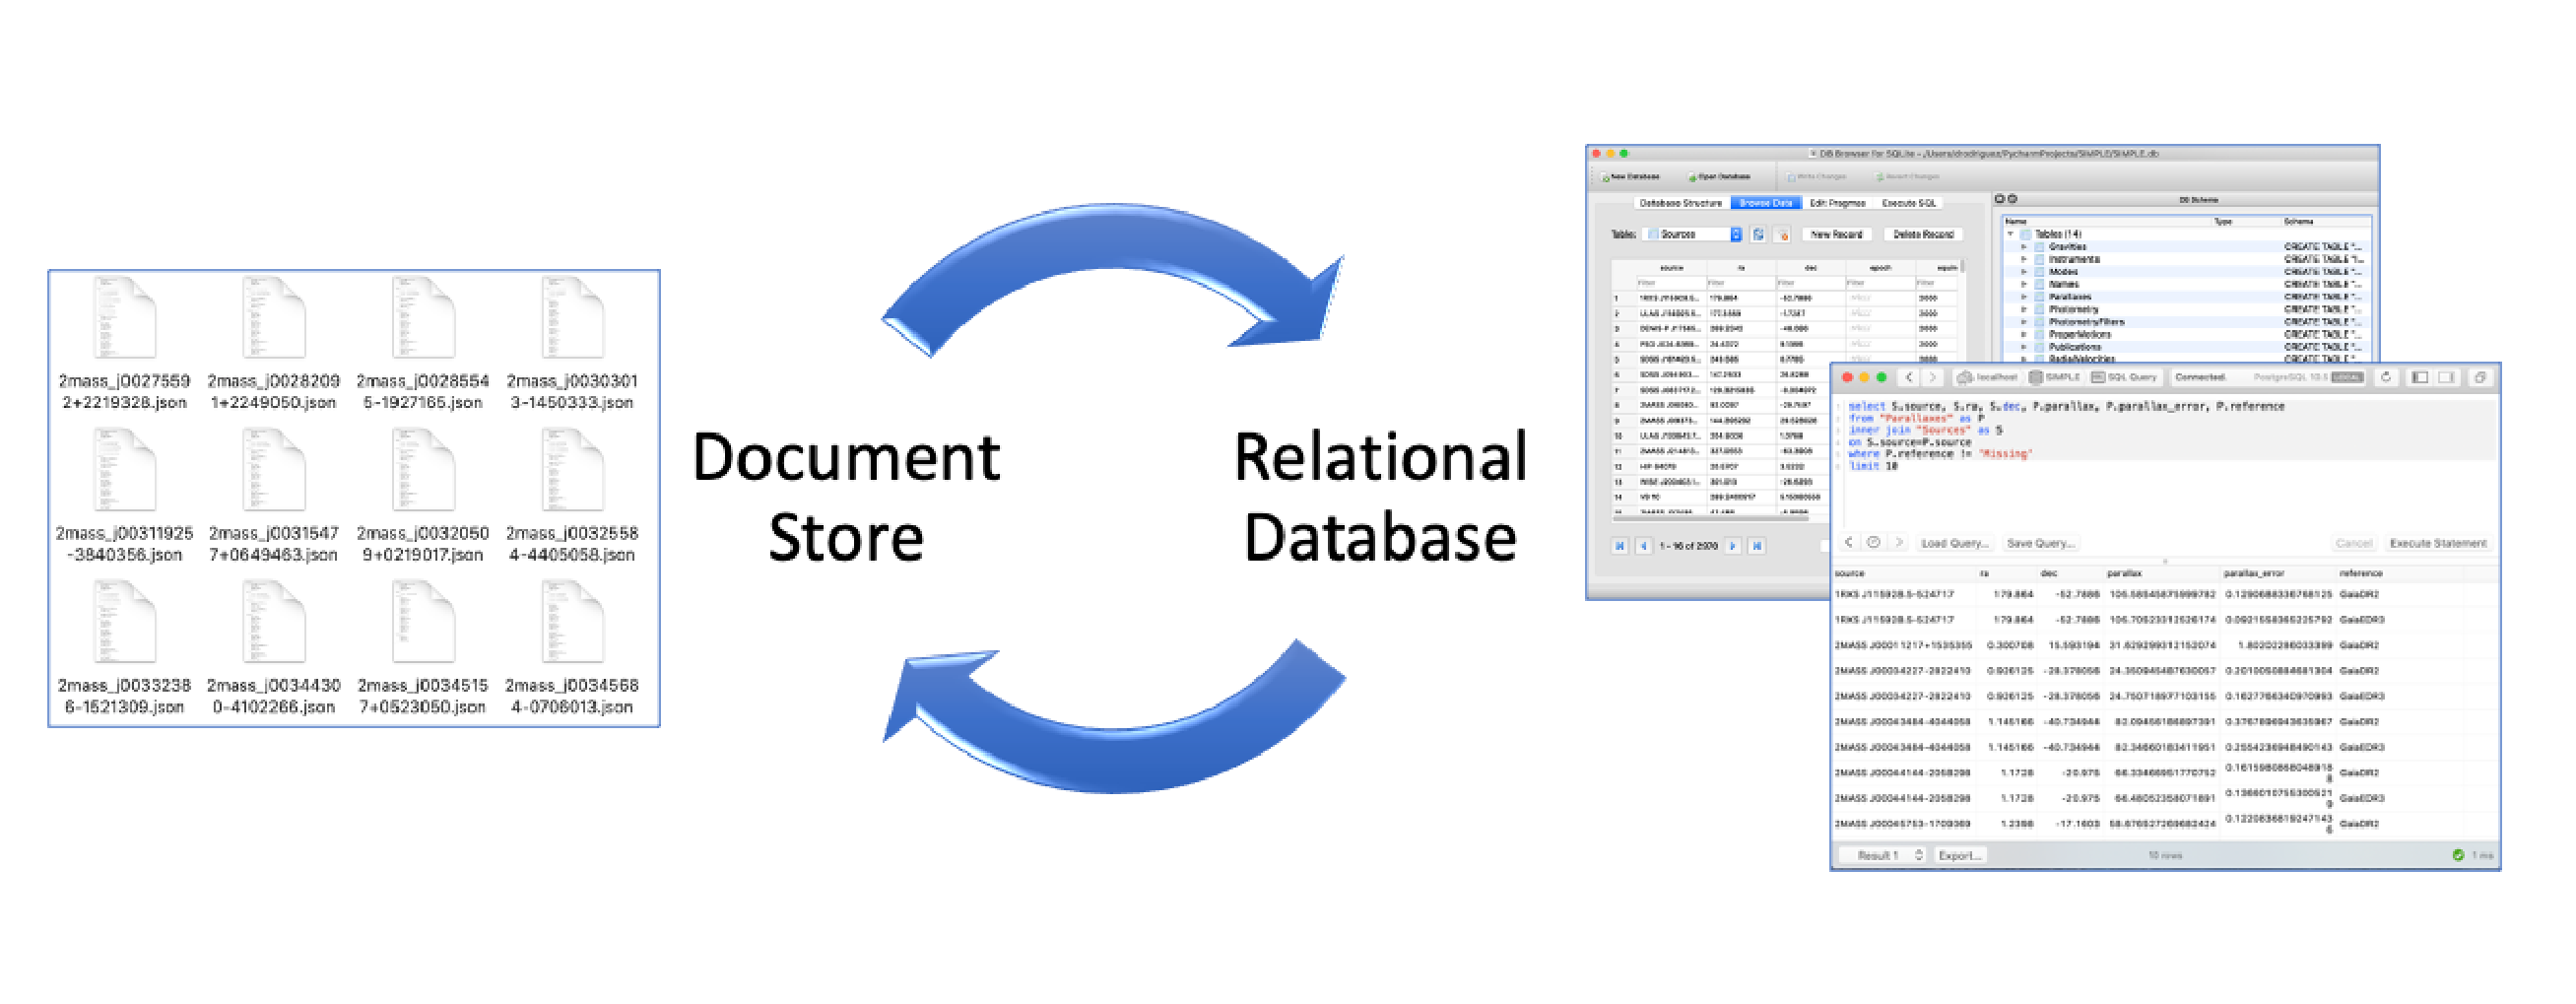
\includegraphics[width=\textwidth]{X0-012_f1.eps}
    \caption{AstrodbKit2 can convert a database from a document store representation (e.g. a list of JSON files) to a relational database (e.g. SQLite, Postgres, etc).}
    \label{fig:astrodbkit2}
\end{figure}

\begin{figure}
    \centering
    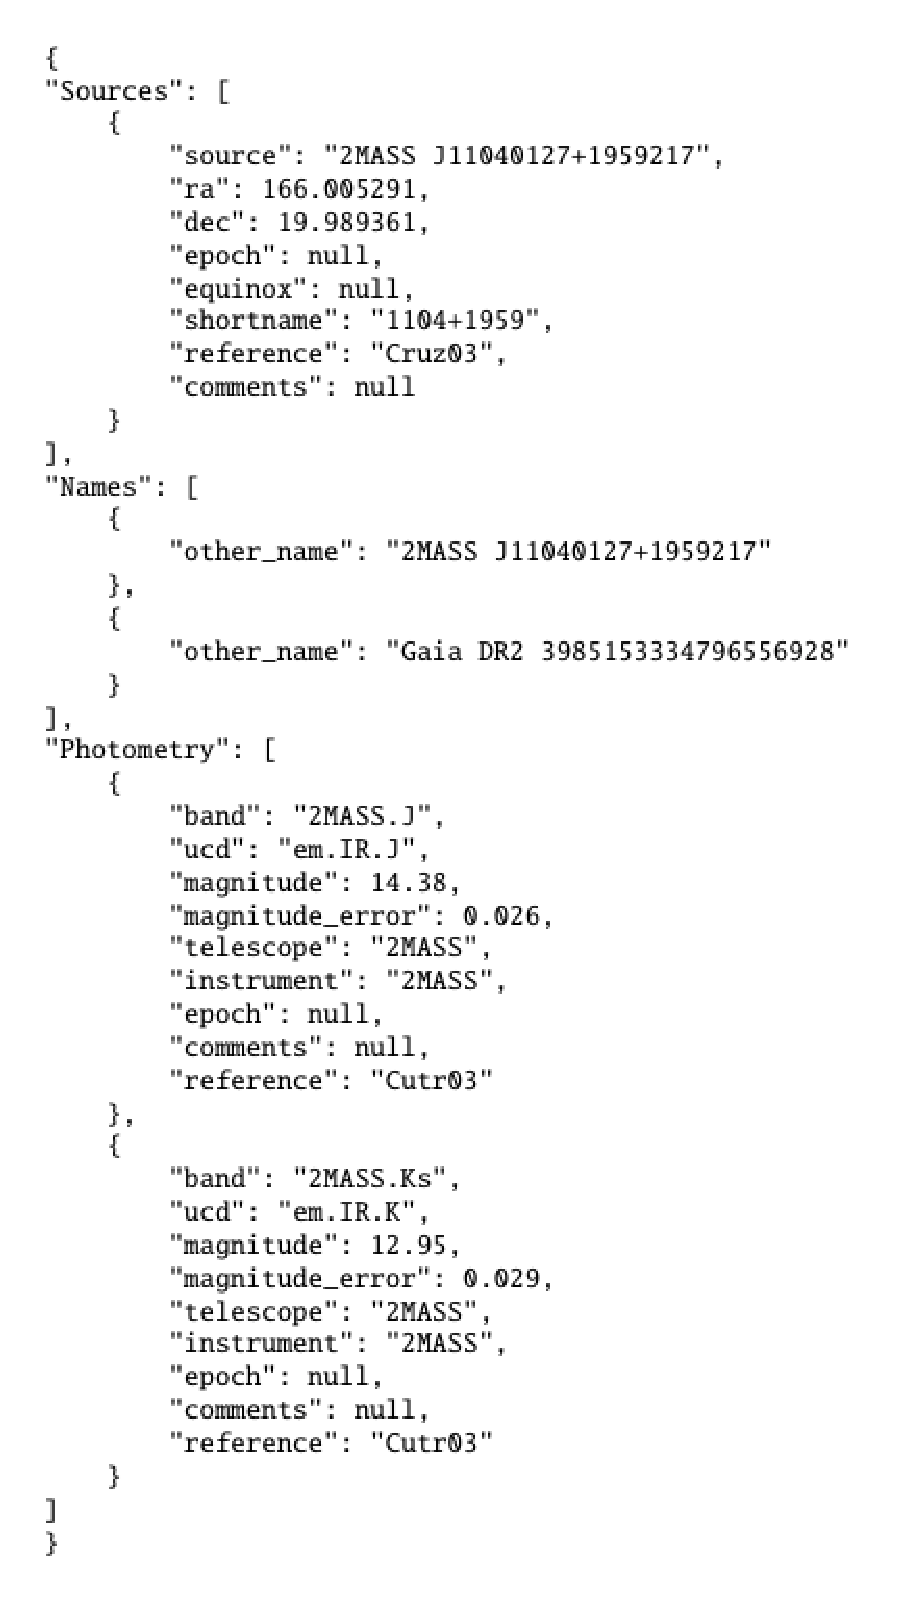
\includegraphics[height=0.9\textheight]{X0-012_f2.eps}
    \caption{Trimmed JSON document for a source in the SIMPLE database}
    \label{fig:json}
\end{figure}

\begin{figure}
\begin{center}
\epsscale{1.2}
\plotone{f2.eps}
\caption{\label{fig:inventory}To search for records and check the data inventory of sources, the \texttt{db.search()} and \texttt{db.inventory()} methods can be used. The first two lines of the example show how \texttt{astrodbkit} is imported and the database is initialized given a file path. Any table can be searched by providing a string, integer, or coordinates to the \texttt{db.search()} method along with a table name. In this example we search the \texttt{SOURCES} table for records that contain the string '0047' and two are found: one with the \texttt{shortname} '0251+0047' and another with '0047+6803'. We can then see all the data that is available for a given source by passing the \texttt{id} from the SOURCES table (in this case 1722) to the \texttt{db.inventory()} method.}
\end{center}
\end{figure}


% END FIGURES ==============================================

\bibliographystyle{aj}
\bibliography{biblio.bib}

\end{document}






















